\documentclass{article}
\usepackage[utf8]{inputenc}
\usepackage[inline]{enumitem}
\usepackage{float}
\usepackage{subcaption}
\usepackage{array}
\usepackage{colortbl}
\usepackage{wrapfig}
\usepackage{multirow}
\usepackage{hulipsum}
\usepackage{graphicx}
\usepackage{xcolor}
\newlist{enuma}{enumerate}{5}
\setlist[enuma]{label=\alph*)}

\begin{document}
	\begin{titlepage}
		\title{\Huge{Bevezetés a \LaTeX-be}}
		\author{\textit{Harmadik alkalom}}
		\date{}
		\maketitle
	\end{titlepage}
	\ref{fig:kepek} \ref{kep2} \subref{kep2} \ref{list2}\ref{list1}
	\section{Bevezetés}
	\begin{itemize}
		\item[*] egy
		\item[*] kettő
		\item[és] három
	\end{itemize}
	\ref{noszam} \ref{szam}
	\begin{enuma}
		\item  plain text after a list as you can see
		\item egy
		\begin{enuma}
			\item  plain text after a list as you can see
			\item[] \label{noszam} ketto
			\begin{enuma}
				\item  plain text after a list as you can see
				\item harom
				\begin{enuma}
					\item kekw
				\end{enuma}
				\begin{enuma}
					\item  plain text after a list as you can see
					\item \label{szam} negy
					\begin{enuma}
						\item  plain text after a list as you can see
						\item ot
					\end{enuma}
				\end{enuma}
			\end{enuma}
		\end{enuma}
	\end{enuma}
	\begin{description}[style=unboxed]
		\item \hulipsum[1]
		\begin{figure}[bt]
			\centering
			\caption{Felirat/képaláírás}
			\label{fig:kepek}
			\begin{subfigure}{5cm}
				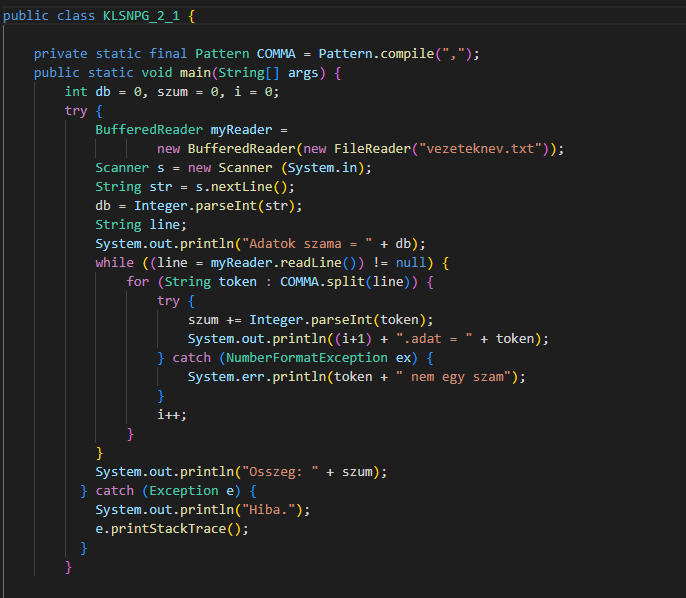
\includegraphics[keepaspectratio, width = 5cm, height = 5cm]{1}
				\hspace{1em} % vízszintes helykihagyás
			\end{subfigure}
			\begin{subfigure}{5cm}
				\caption{lol}
				\label{kep2}
				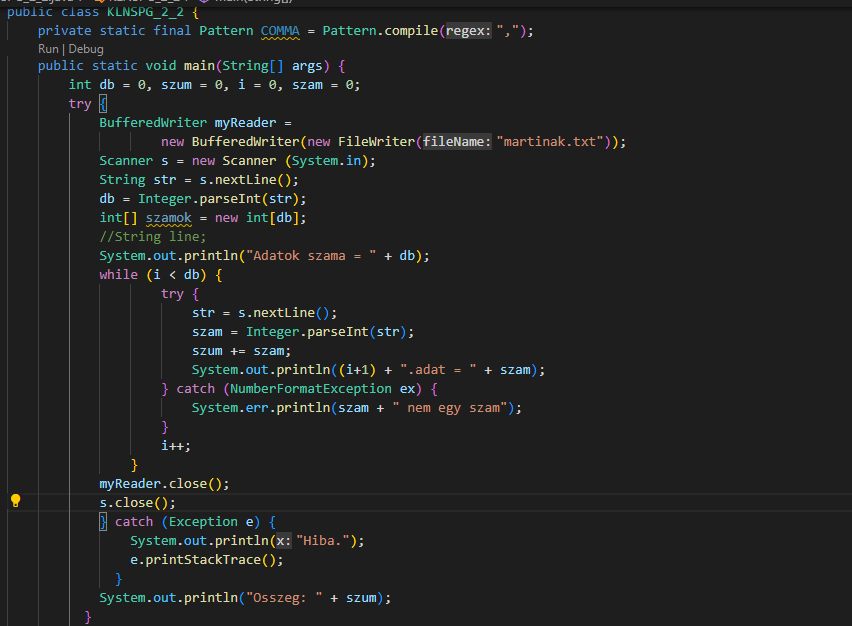
\includegraphics[keepaspectratio, width = 5cm, height = 5cm, angle = 180]{2}
			\end{subfigure}
		\end{figure}
		\item[kicsi] \hulipsum[1]
		\item \hulipsum[1]
		\item[naaaaaaagy] \hulipsum[1]
	\end{description}
	
	\label{list1}
	\begin{tabular}{c||ccc|}
		& egy & ketto & harom \\ \hline
		\multirow{2}{3cm}{Hello\\volág} & negy & ot & het \\ 
		&  &  &  \\ \cline{2-4}
		& het  & nyolc & kilenc\\ \cline{2-2} \cline{4-4}
		\multirow{2}{3cm}{lorum\\ipse}& tiz & & tizengy \\ 
		& & & \\\hline
	\end{tabular}
	
	\label{list2}
	\begin{tabular}{||ccc|}
		\rowcolor{cyan}
		egy & ketto & harom \\ \hline
		\rowcolor{cyan}
		negy & ot & het \\ 
		\rowcolor{red}
		&  &  \\ \cline{1-3}
		\rowcolor{red}
		het  & nyolc & kilenc\\ \cline{1-1} \cline{3-3}
		\rowcolor{cyan}
		tiz & & tizengy \\ 
		\rowcolor{cyan}
		& & \\\hline
	\end{tabular}
	
	
	\label{list3}
	\begin{tabular}{r!{\color{red}\vline}cc|}
		egy & \multicolumn{2}{c|}{ketto}\\ \hline
		\multirow{2}{1cm}{negy} & öt \vline& hat\\ \cline{2-3}
		& \multicolumn{2}{c|}{\multirow{2}{1cm}{nyolc}}\\ \cline{1-1}
		tiz & &\\ \hline
	\end{tabular}
	
\end{document}